This chapter outlines the methods and techniques employed in the development of a conversational question-answering system designed for PDFs. The chapter is structured as follows: Section \ref{sec:overview} provides an overview of the desired use case, its objectives, and constraints concerning a Conversational Question Answering System. Section \ref{sec:conrag} presents a general framework that can be utilized as a decision tree for the practical implementation of a Conversational Question Answering System for PDFs. Its subsections will highlight and discuss the components introduced within the framework.

\section{Overview and Objective}
\label{sec:overview}

The primary use case addressed in this thesis can be summarized as follows: Imagine having a collection of PDF files, and our goal is to create a chatbot capable of engaging in conversations about the knowledge within these PDFs. This chatbot should provide accurate answers to questions based on the content of the PDFs and furnish supporting evidence from these documents. Furthermore, it should enable users to have a conversational query experience, allowing them to ask follow-up questions and engage in dialogue with the chatbot based on its previous responses. Figure \ref{fig:use-case} illustrates an example of this use case.

\begin{figure}
    \centering
    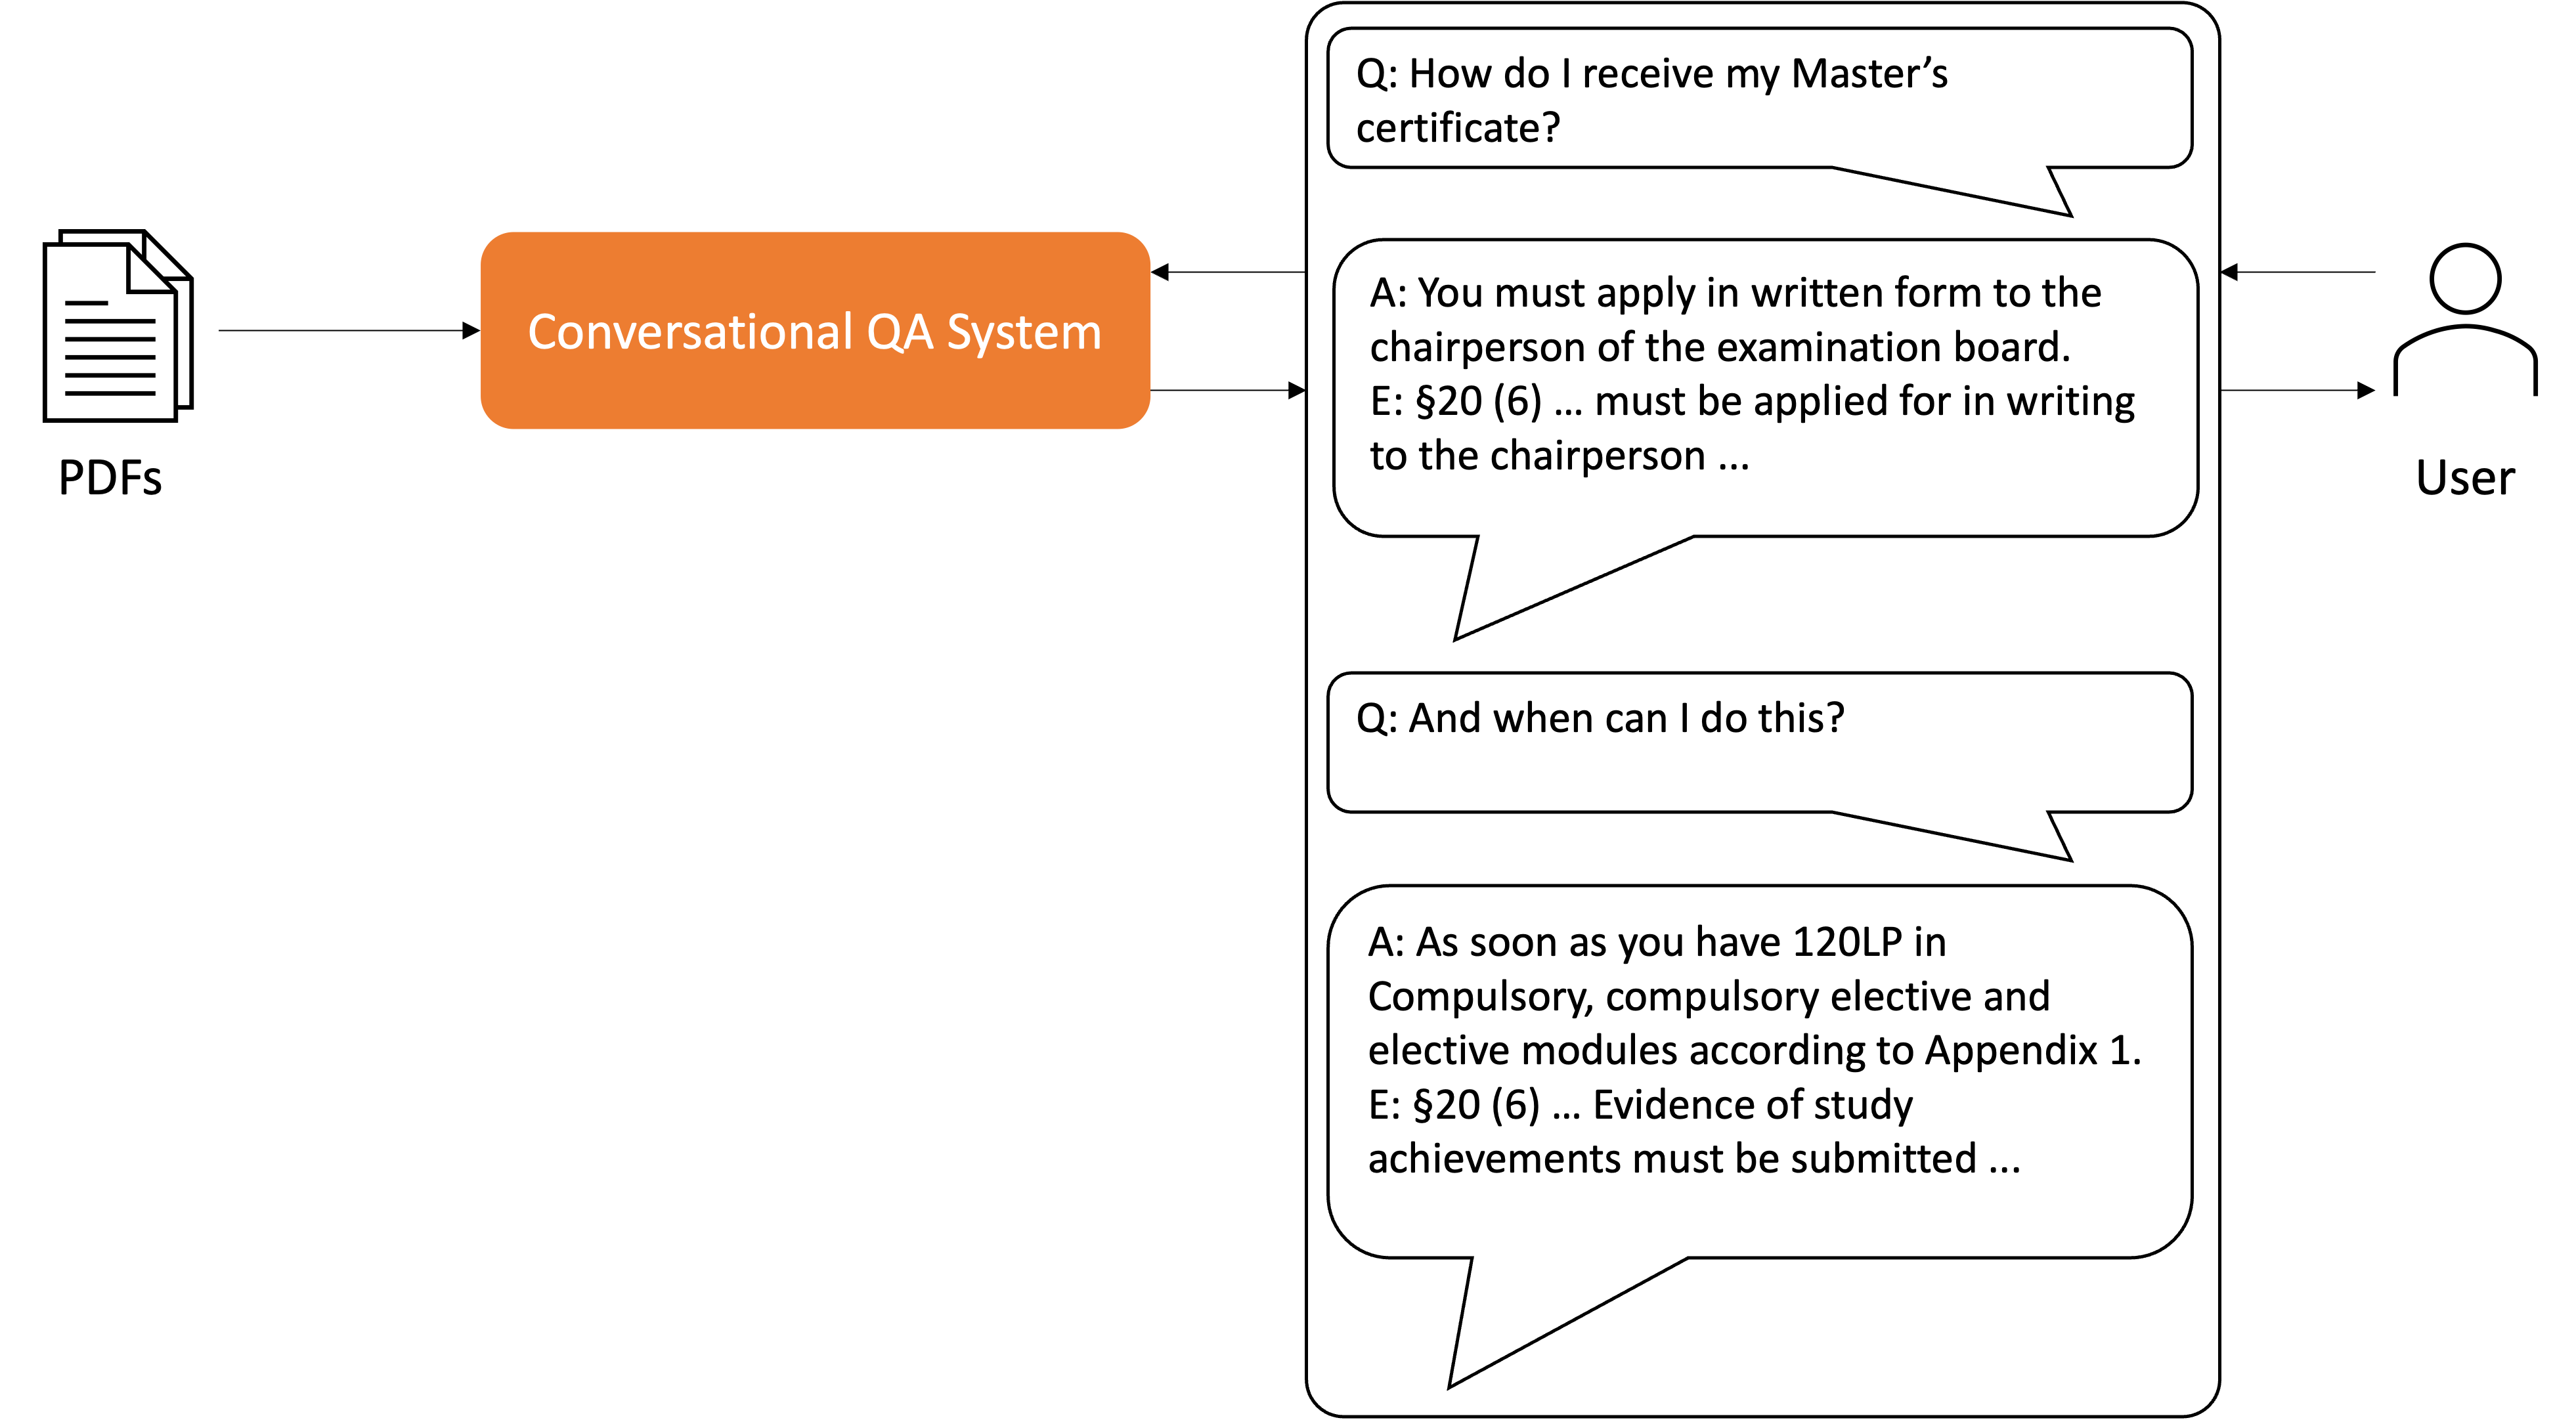
\includegraphics[width=0.8\textwidth]{Grafiken/Use_Case.png}
    \caption{Overview of the Example Use-Case}
    \label{fig:use-case}
\end{figure}

Currently, to the best of my knowledge, there is no scientific paper or similar resource offering a comprehensive framework or pipeline to address this use case. This thesis aims to bridge this gap by presenting a framework and pipeline designed to tackle this specific scenario. Figure \ref{fig:overview-system-architecture} provides an overview of the system architecture. The system follows the \gls{rag} architecture, as detailed in Section \ref{subsec:qa_retrieval}, which extends the classical Retriever-Reader with a \gls{llm} as a Reader, capable of incorporating parametric knowledge. To extend \gls{rag} to a \gls{convqa}, a \gls{cqu} unit, as introduced in Section \ref{subsec:cqa_contextual_query_understanding}, is essential. This novel architecture will be termed \textbf{\gls{conrag}}. The extraction pipeline will be discussed in Section \ref{subsec:extract}, with its primary tasks being the extraction of passages from the provided set of PDFs, the creation of an index, and the optional generation of synthetic training data. The three major modules comprising the architecture, namely the \textit{Retriever}, \textit{Reader}, and \textit{\gls{cqu}}, will be elaborated in their respective sections: \ref{subsec:retriever}, \ref{subsec:reader}, and \ref{subsec:cqu}.

\begin{figure}
    \centering
    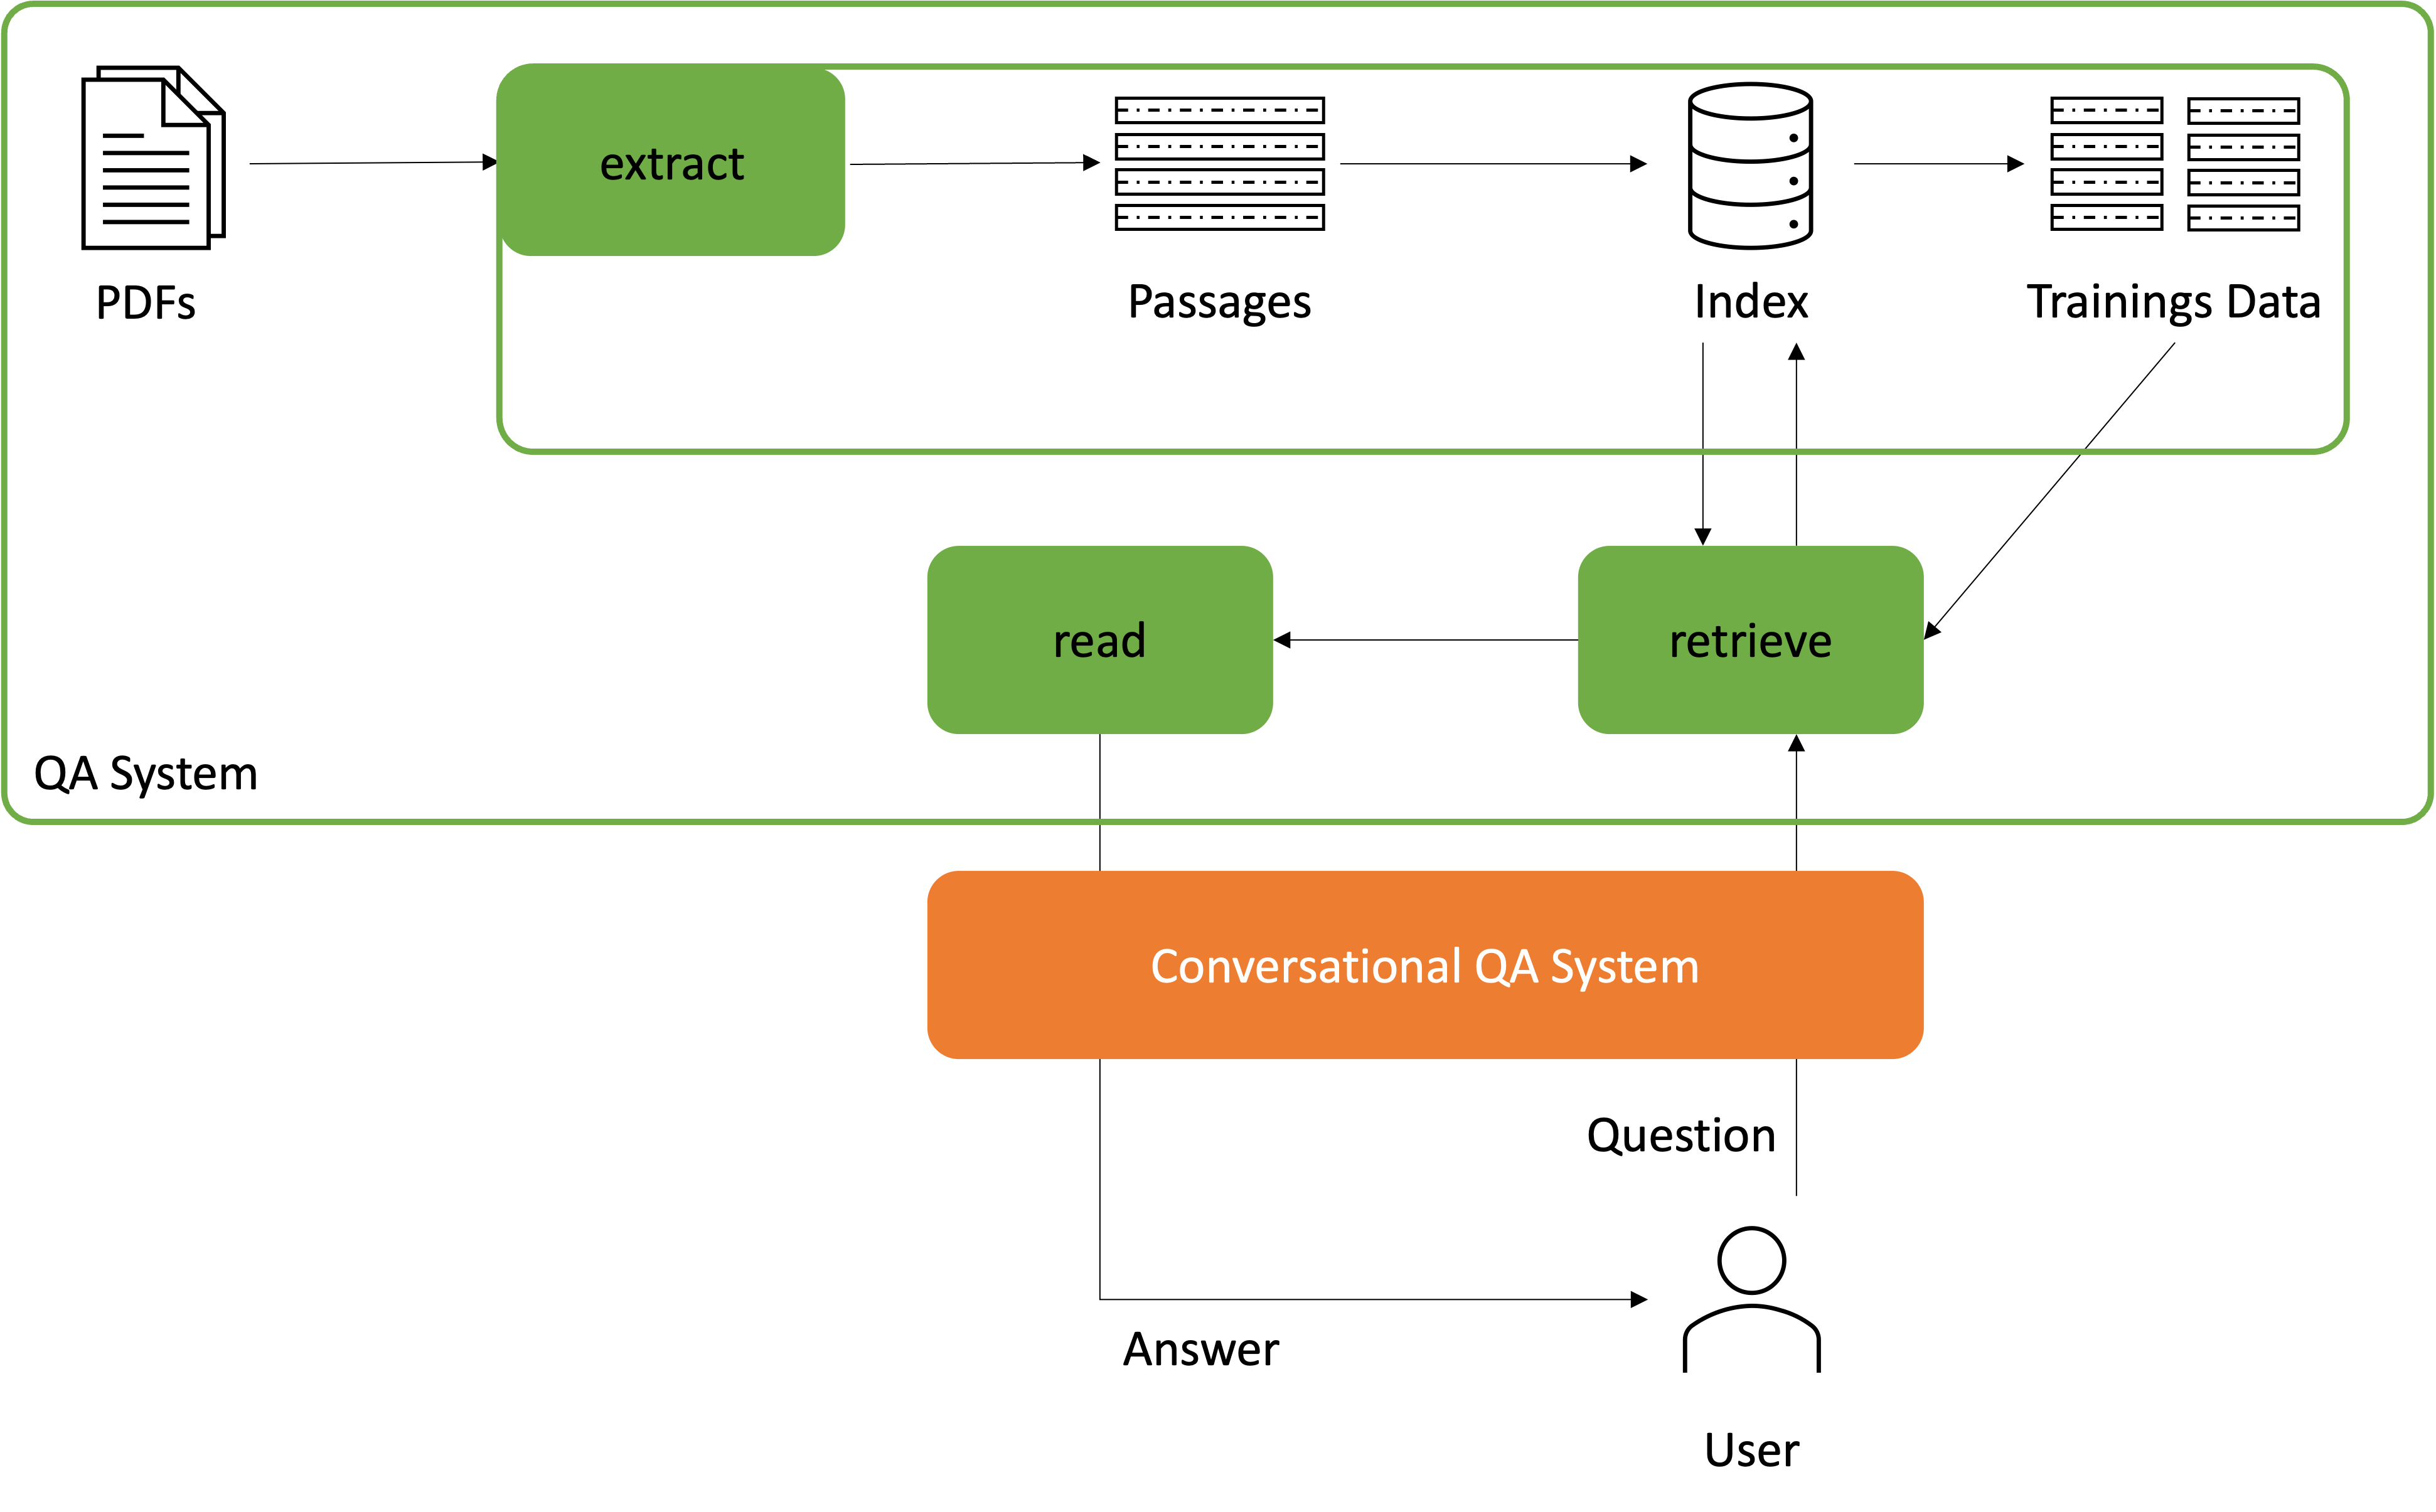
\includegraphics[width=0.8\textwidth]{Grafiken/System_Architecture.png}
    \caption{Overview of the System Architecture}
    \label{fig:overview-system-architecture}
\end{figure}

To summarize, the objectives of the QA capabilities of the system are as follows:

\begin{enumerate}
    \item Utilize \textbf{PDFs} as the primary \textbf{knowledge source}.
    \item Enable the QA-System to handle a \textbf{variety of question types}, including: \textbf{extractive}, \textbf{abstractive}, and \textbf{boolean questions}.
    \item \textbf{Provide references} to PDF snippets \textbf{as evidence to answers}.
    \item Ensure the pipeline's generalizability, allowing it to adapt to new domains or knowledge sources with \textbf{minimal or no supervision} and \textbf{small datasets}.
    \item Design the pipeline to be \textbf{feasible without the need for datacenter-grade hardware resources}, making it accessible for development on standard research hardware.
    \item \textbf{Prioritize accuracy as the primary objective}, as constraining memory consumption is indirectly covered in point (5). \textbf{Latency is not a primary concern}, as the system is not intended for real-time use and will not be optimized for that.
\end{enumerate}


Regarding the ConvQA-System, the objectives are as follows:

\begin{enumerate}
    \item Enable the ConvQA-System to \textbf{handle} the following follow-up \textbf{question types: drilling-down, clarification, topic shift} and \textbf{comparison}.
    \item Be able to take Initiative in the form of \textbf{clarifying questions}.
    \item The \textbf{memory} will be \textbf{limited to a session}.
\end{enumerate}

\section{Conversational Retrieval-Augmented Generation}
\label{sec:conrag}

As illustrated in Figure \ref{fig:overview-system-architecture}, it is logical to partition the extensive grid of possibilities into smaller, manageable components that can be explored and designed independently. Consequently, the framework will be divided into two main segments: the extraction pipeline, with its potential configurations outlined in Figure \ref{fig:extract_pipeline}, and the three major modules: Retriever, Reader, and \gls{cqu}, showcasing their possible implementations in Figure \ref{fig:all_components_conrag}.

\begin{figure}
    \centering
    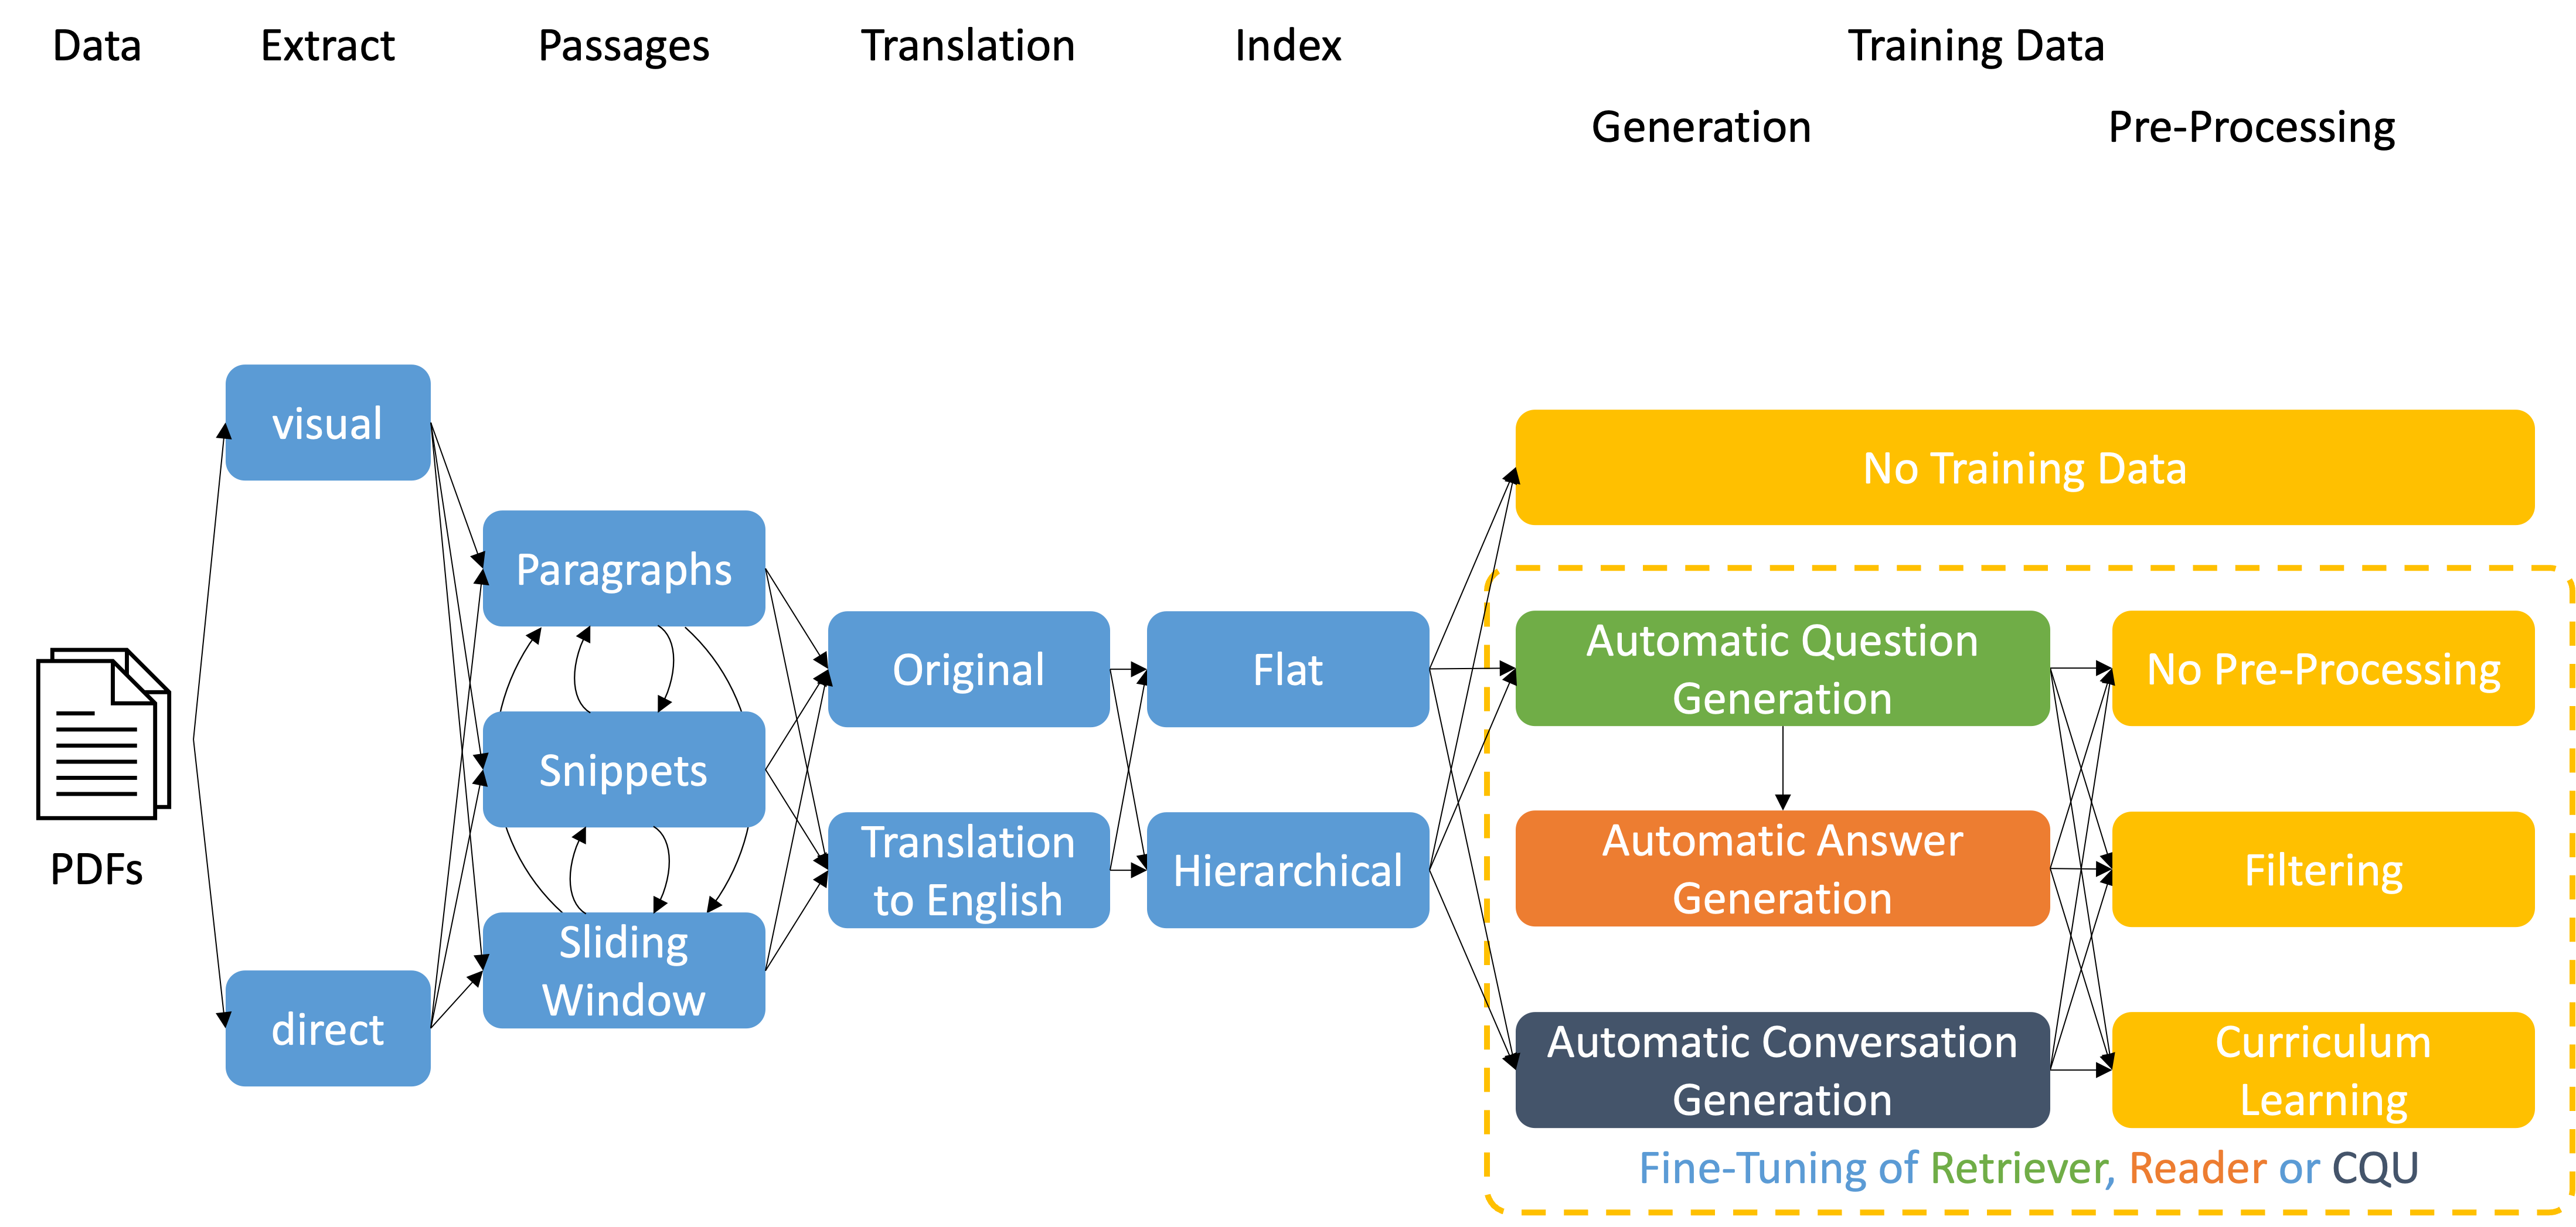
\includegraphics[width=\textwidth]{Grafiken/extract_pipeline.png}
    \caption{Overview of the Extraction Pipeline Framework}
    \label{fig:extract_pipeline}
\end{figure}

The framework varies in its level of granularity, shifting between high-level concepts and precise details. This is primarily due to the fact that certain aspects of the framework are well-researched and represent state-of-the-art knowledge, while others are ongoing research and necessitate a more abstract, conceptual treatment. For instance, \textit{BM25} is mentioned specifically as the state-of-the-art Sparse Retriever within the Retriever Module, whereas \textit{Automatic Question Generation} in the Training Data Generation step of the extraction pipeline is presented as a high-level concept.

The framework strives to maintain a high level of generality, intentionally avoiding the incorporation of restrictive paradigms, except for the specified system architecture of \gls{rag} for \gls{qa}. This decision is motivated by the burgeoning breakthroughs and extensive research endeavors within the field of \gls{llm}s, as exemplified by the exceptional success of \textit{ChatGPT}. In response to the limitations of ChatGPT, including \textit{hallucination}, \textit{implicit knowledge}, and \textit{knowledge update}, interest has surged in the \gls{rag} architecture as a means to address these issues. Presently, there is no existing survey or similar resource that provides a quantitative evaluation of the ongoing business initiatives aimed at implementing RAG-based Systems. Nonetheless, both Google Cloud Services \cite{noauthor_generative_nodate} and Amazon Web Services \cite{noauthor_quickly_2023} have introduced new services that empower customers to construct \gls{rag}-based systems, with Langchain serving as the Framework for the Reader Implementation\cite{noauthor_langchain-ailangchain_nodate}. Consequently, the framework presented here seeks to illuminate potential pathways for implementing a \gls{conrag} system, as depicted in Figure \ref{fig:convqa_system_architecture}, tailored to the use case described in Section \ref{sec:overview}.

The extraction pipeline can be visualized as a tree, where following different paths signifies making decisions with corresponding implications for subsequent steps and components. In Figure \ref{fig:all_components_conrag}, each column represents a decision to be made, although in some cases, choosing not to decide is itself a decision. Dotted lines encircling multiple frames indicate that a combination or ensemble approach is possible. For a better understanding of how to apply this framework to create a potential system implementation, refer to the example in Figure \ref{fig:example_decission_tree}. As previously mentioned, the framework does not prescribe specific models (e.g., BERT, PaLM, etc.) but rather conceptual approaches (e.g., Cross-Encoder). The example in Figure \ref{fig:example_decission_tree} represents a simple zero-shot baseline, which will also be implemented and tested in this thesis Chapter \ref{chap:eval}.

\begin{figure}
    \centering
    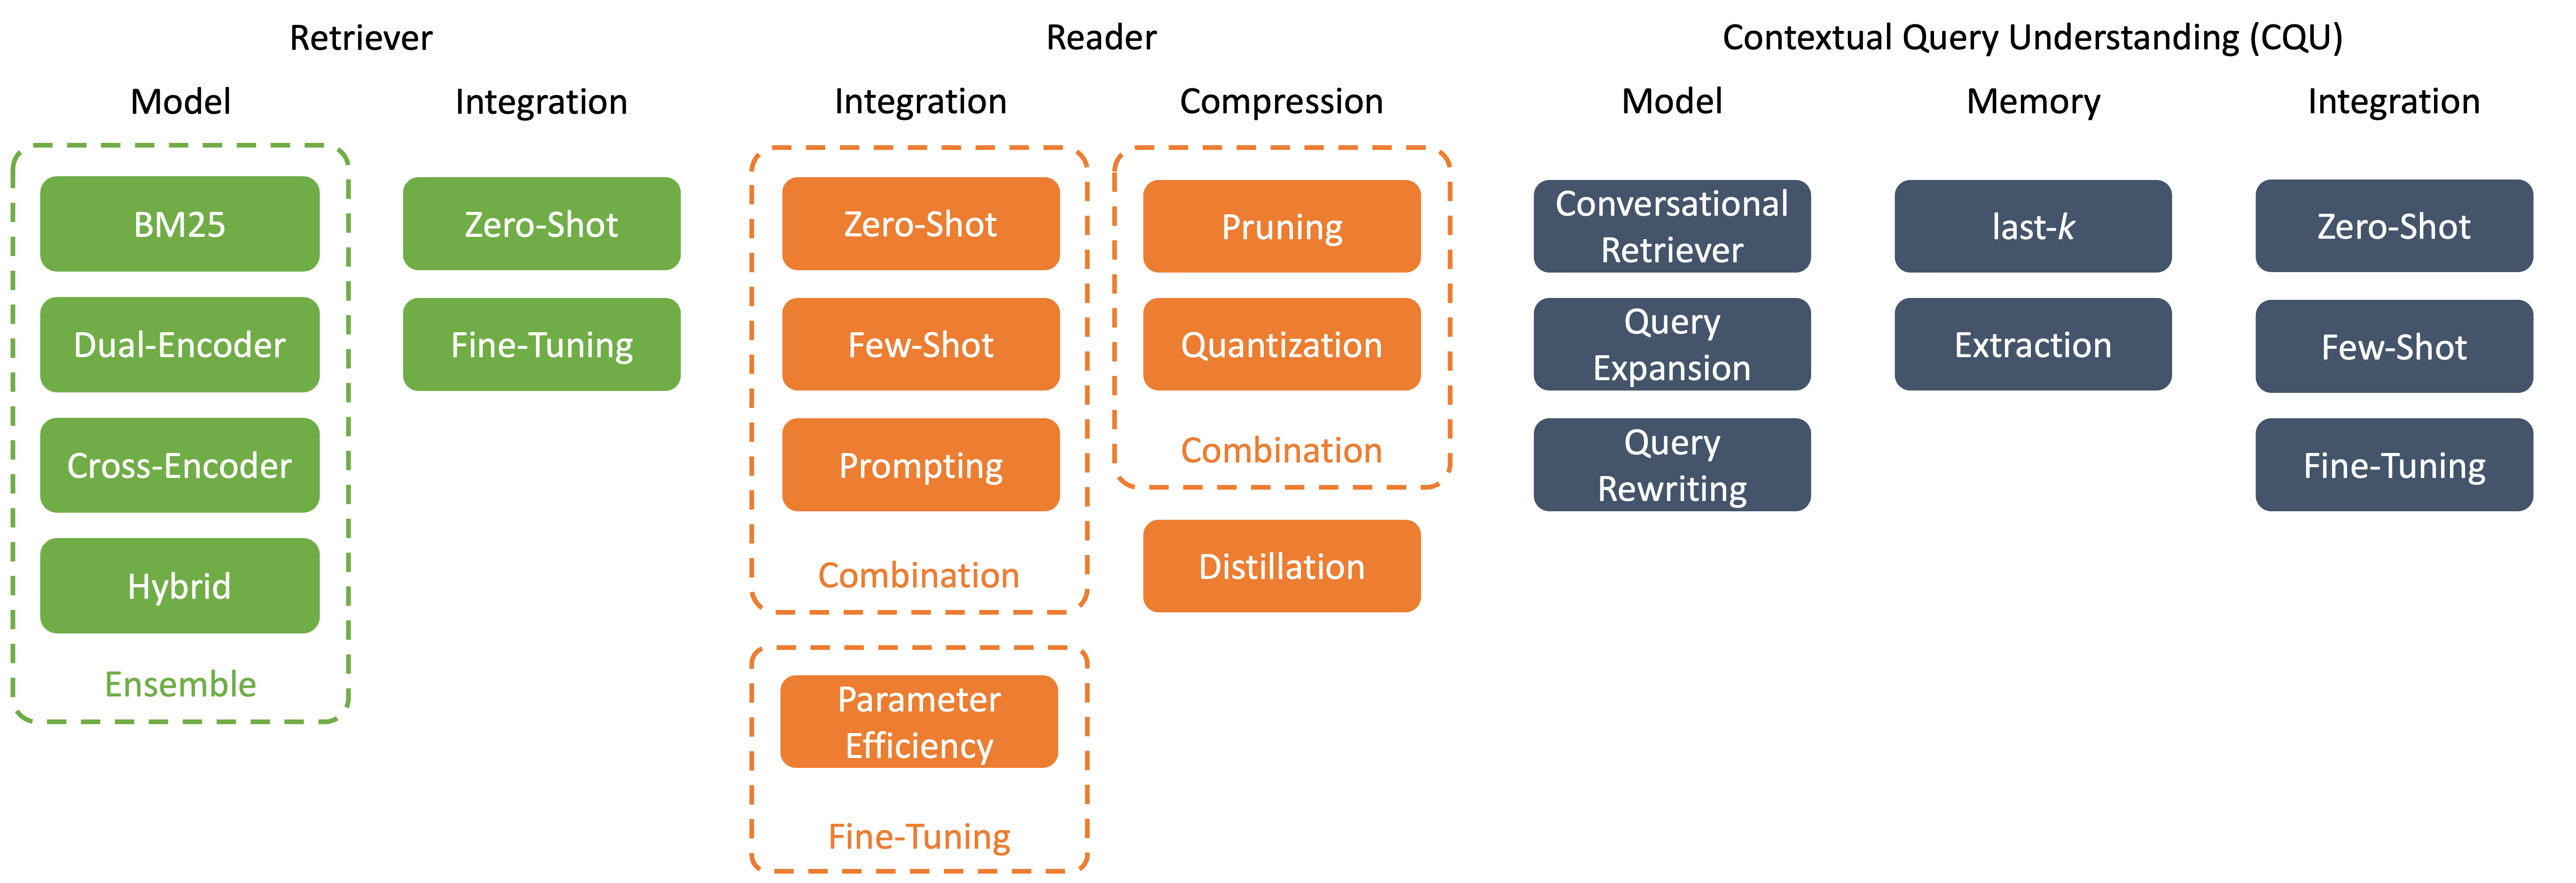
\includegraphics[width=\textwidth]{Grafiken/all_components_conrag.png}
    \caption{Overview of all Modules of the Framework}
    \label{fig:all_components_conrag}
\end{figure}

\begin{figure}
    \centering
    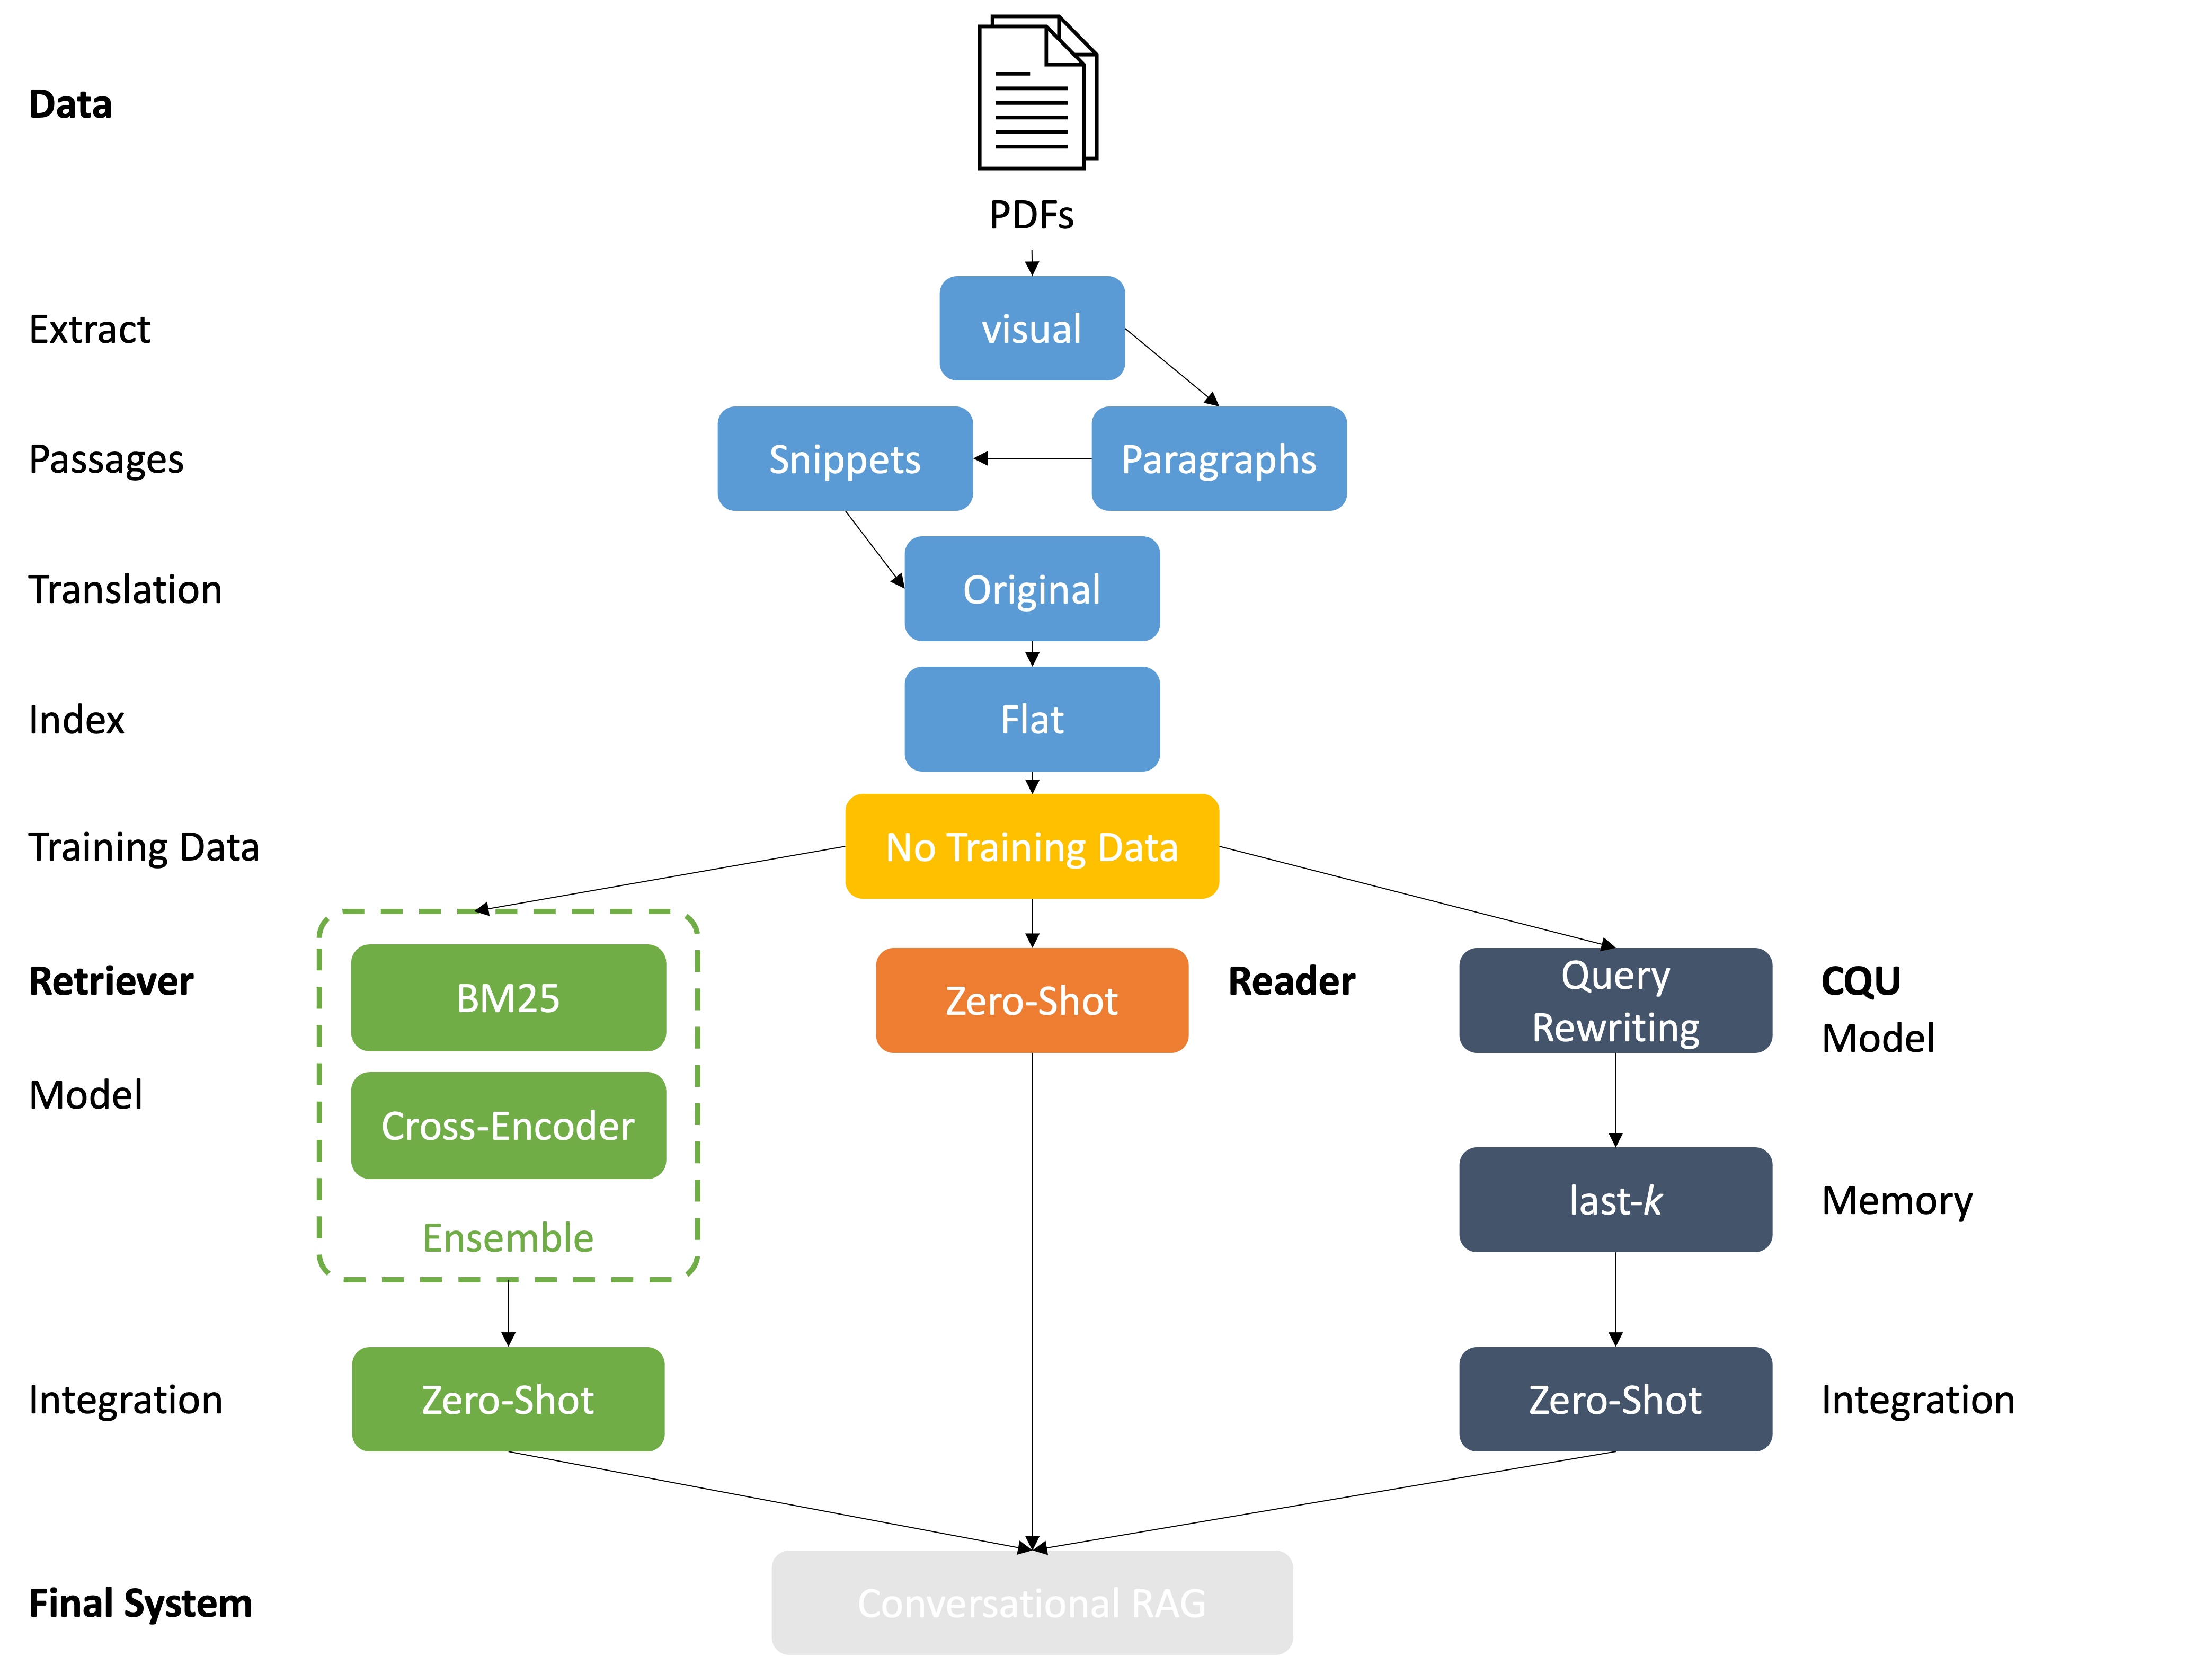
\includegraphics[width=\textwidth]{Grafiken/example_decission_tree.png}
    \caption{Example of applying the Framework to a System Implementation}
    \label{fig:example_decission_tree}
\end{figure}



\subsection{extract}
\label{subsec:extract}

\subsection{Retriever}
\label{subsec:retriever}

\subsection{Reader}
\label{subsec:reader}

\subsection{Contextual Query Understanding}
\label{subsec:cqu}


% \section{Question Answering over PDFs}
% \label{sec:qa-over-pdfs}

% \begin{figure}
%     \centering
%     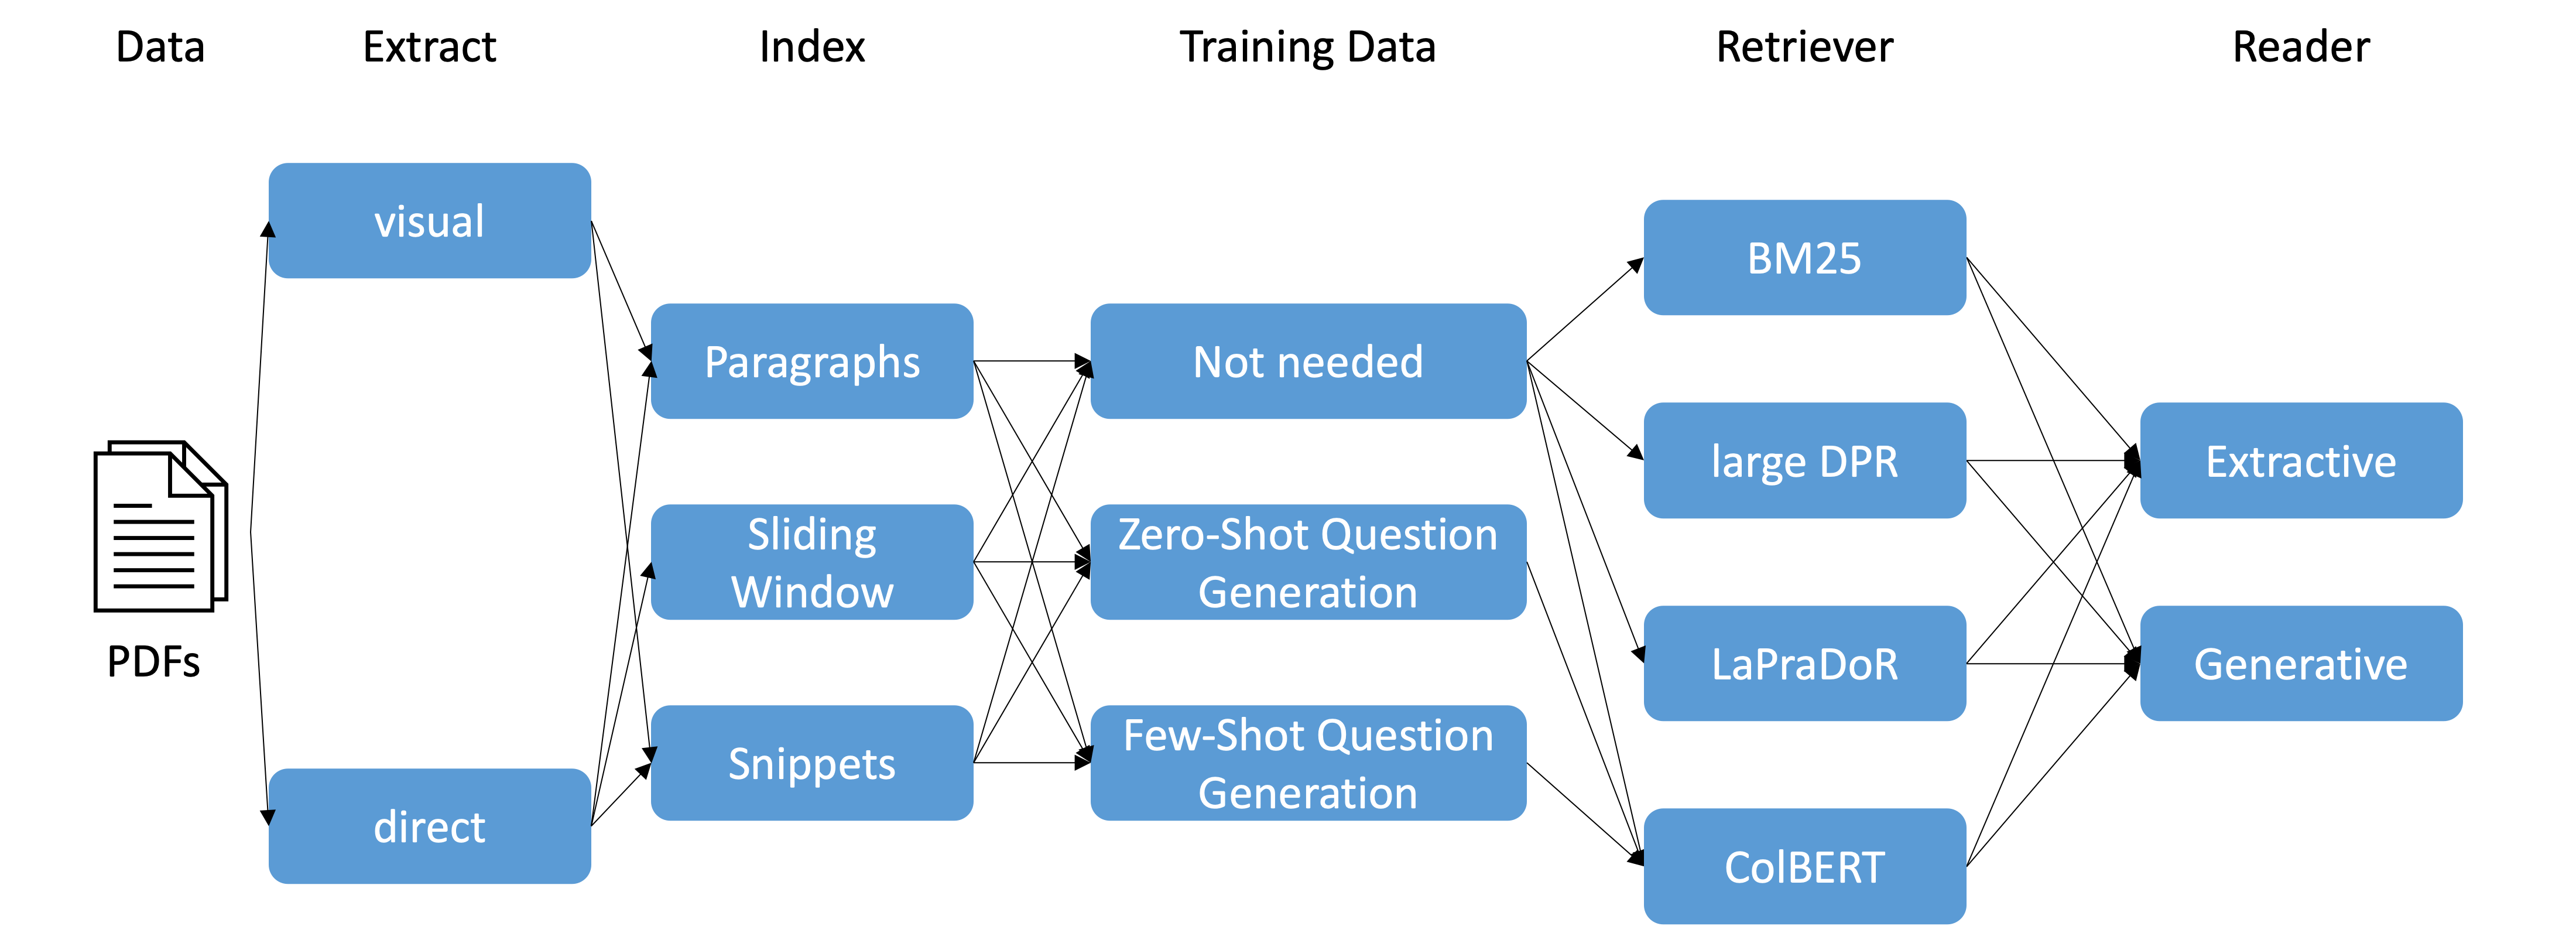
\includegraphics[width=0.8\textwidth]{Grafiken/Possible_Systems.png}
%     \caption{Possible Combinations of Modules to Create an Adapted QA-System}
%     \label{fig:qa-system-combinations}
% \end{figure}

% The possible combinations of modules to create an adapted \gls{qa}-System can be seen in Figure \ref{fig:qa-system-combinations}.


% \subsection{Extract}
% \label{subsec:extract}

% \textbf{Information Extraction:} When it comes to extracting text from PDFs, you have two approaches to choose from: the \textit{visual} approach and the \textit{direct} approach, each with its own advantages. In the \textit{visual} approach, you can create a model for document layout analysis combined with an OCR tool. Ideally, this approach yields a collection, denoted as $M$, comprising paragraphs $m$. These paragraphs vary in length but represent self-contained semantic units from the underlying PDF. On the other hand, the \textit{direct} approach is suitable only for digitally-born PDFs. For such PDFs, you can employ a tool like Py2PDF \cite{noauthor_welcome_nodate}. This results in a corpus $M$ that requires processing to achieve the desired granularity.

% \noindent\textbf{Indexing:} The implementation of indexing depends on the nature of $M$ and the desired granularity of the output. In general, there are three approaches to constructing passages $p$ in the index $P$:

% \begin{enumerate}
%     \item \textit{Paragraphs:} In this approach, $P$ comprises passages $p_i$ such as $P = \{p_1, p_2, \ldots, p_n\}$, where each $p_i$ is derived from $M$ and represents semantic paragraphs from the original document. The length $l$ of each $p_i$ is not fixed, and the number of paragraphs $|P|$ can also vary.
%     \item \textit{Snippets:} When you have a fixed passage length $l$, the concatenated text corpus $M$ is divided into $|M|\bmod{l} + 1$ passages $p$. Alternative approaches may involve specifying minimum and maximum lengths, denoted as $l_{\text{min}}$ and $l_{\text{max}}$. The exact point of division depends on whether a sentence ends within the specified window or not. If a sentence ending is found within the window, the snippet concludes at that point; otherwise, it concludes at the end of the window.
%     \item \textit{Sliding Windows:} This approach utilizes a window size $l$, a concatenated text corpus $M$, and a step size $s$. The window slides over the text corpus $M$, and the text within the window is used as a passage $p$. This results in $\frac{|M| - l}{s}$ passages, denoted as $P = \{p_1, p_2, \ldots, p_n\}$.
% \end{enumerate}

% \textit{Paragraphs} may seem like the most intuitive choice, but the indefinite length of passages, denoted as $p$, can be an issue. \textit{Snippets} have the advantage of having almost uniform lengths. However, a downside could be that important connections between sentences are lost, potentially leading to the loss of information. \textit{Sliding Windows} offer the advantage of uniform lengths and the ability to capture connections between sentences. However, the downside is the high number of passages, denoted as $p$, that need to be indexed, along with potential issues related to data cleanliness.

% \noindent\textbf{Synthetic Training Data Generation:} In this pipeline, the prompt-based \gls{qg} method known as PROMPTAGATOR \cite{dai_promptagator_2022} is used to generate a synthetic \gls{qa} dataset for ColBERTv2 \cite{santhanam_colbertv2_2022} based on $P$. The goal is to create triples of $(q, p^{+}, p^{-})$, similar to those found in datasets like MS MACRO \cite{bajaj_ms_2018}. For the task of $E_{qg}(p) := q$, a \gls{s2s} model, specifically a \gls{llm}, will be employed. This technique can be interpreted as knowledge distilation from the LLM to the later trained retriever. Similar to PROMPTAGATOR, there are two approaches to consider:

% \begin{enumerate}
%     \item \textit{Zero-Shot:} In this approach, a single prompt is executed to generate a question $q_i$ corresponding to a passage $p_i$, all without the need for any supervised dataset.
    
%     \item \textit{Few-Shot:} This approach uses $k$ supervised pairs $(q_j, p^{+}_{j})^{k}$ to generate a question $q_i$ corresponding to a passage $p_i \in P$.
% \end{enumerate}

% The prompt used for \textbf{zero-shot \gls{qg}}, where $p_i$ represents a passage from $P$, is:

% \verb|f'{p_i} Read the passage and generate a corresponding query.'|

% The prompt used for \textbf{few-shot \gls{qg}}, where $q_j$ represents a question, $p_j$ the corresponding passage, and $p$ the passage for which a question is being generated, is:

% \verb|f'Passage: {p_1} Question: {q_1} XXX Passage: {p_2} Question: {q_2}|

% \verb|XXX ... XXX Passage: {p} Question:'|

% The result of either of these approaches will be a synthetic training dataset of $(q_s, p^{+})$ tuples. This dataset can be used for fine-tuning the retriever.

% A major issue associated with this form of \textbf{\gls{qg}} is its strict limitation to extractive questions, where the evidence can be derived from a single passage only. This limitation significantly constrains this pipeline. However, it does not necessarily prevent the system from answering more complex questions, such as multi-hop questions. These can be addressed by the \textit{retriever} and \textit{reader} modules.

% %%%%%

% \subsection{Retrieve}
% \label{subsec:retrieve}

% \textbf{Out-of-Domain Retrievers:} The easiest implementation is the out-of-domain usage of retrievers without fine-tuning and the need for generating a training dataset. Three major retrievers seem promising due to their performance on the BEIR \cite{thakur_beir_2021} out-of-domain benchmark for retrievers:

% \begin{enumerate}
%     \item \textit{BM25} is the standard Sparse Retriever based on lexical probabilistic matching between the query $q$ and passages $p$.
%     \item \textit{Large DPRs} are Dense Retrievers based on large encoders. They utilize typical dense retrieval paradigms and are a primary approach in open-source projects like \textit{Langchain} \cite{noauthor_langchain-ailangchain_nodate}.
%     \item \textit{LaPraDoR} is a hybrid retriever based on a broadly trained Representation-based Retriever, similar to (2), combined with lexical weighting (1).
% \end{enumerate}

% The \gls{laprador} utilizes the advantages of both lexical and semantic search. Given a question $q$ and a passage $p$, the semantic similarity $\text{sim}(q,d)$ is calculated using a \gls{dpr} model. In addition, the lexical similarity $\text{BM25}(q,d)$ is calculated. The final score $\text{score}(q,d)$ is computed as follows:

% \begin{equation}
%     \mathbf{score}(q, d) = \mathbf{sim}(q, d) \cdot \mathbf{BM25}(q, d)
% \end{equation}

% This approach achieves state-of-the-art performance on the BEIR benchmark without the need for fine-tuning. It serves as the ideal off-the-shelf component for the desired \gls{qa}-System.

% \noindent\textbf{Fine-Tuning Retrievers:} Fine-tuning is a challenging task in the absence of a supervised dataset, especially when dealing with a Representation-Interaction Retriever like ColBERTv2. Currently, there is no clear reference on how to fine-tune a Representation-Interaction Retriever like ColBERTv2 on synthetic data. To address this gap, this thesis proposes the approach depicted in Figure \ref{fig:retriever-fine-tuning}, which combines elements from the training processes of PROMPTAGATOR \cite{dai_promptagator_2022}, the original \gls{dpr} \cite{karpukhin_dense_2020}, and ColBERTv2 \cite{santhanam_colbertv2_2022}.

% \begin{figure}
%    \centering
%     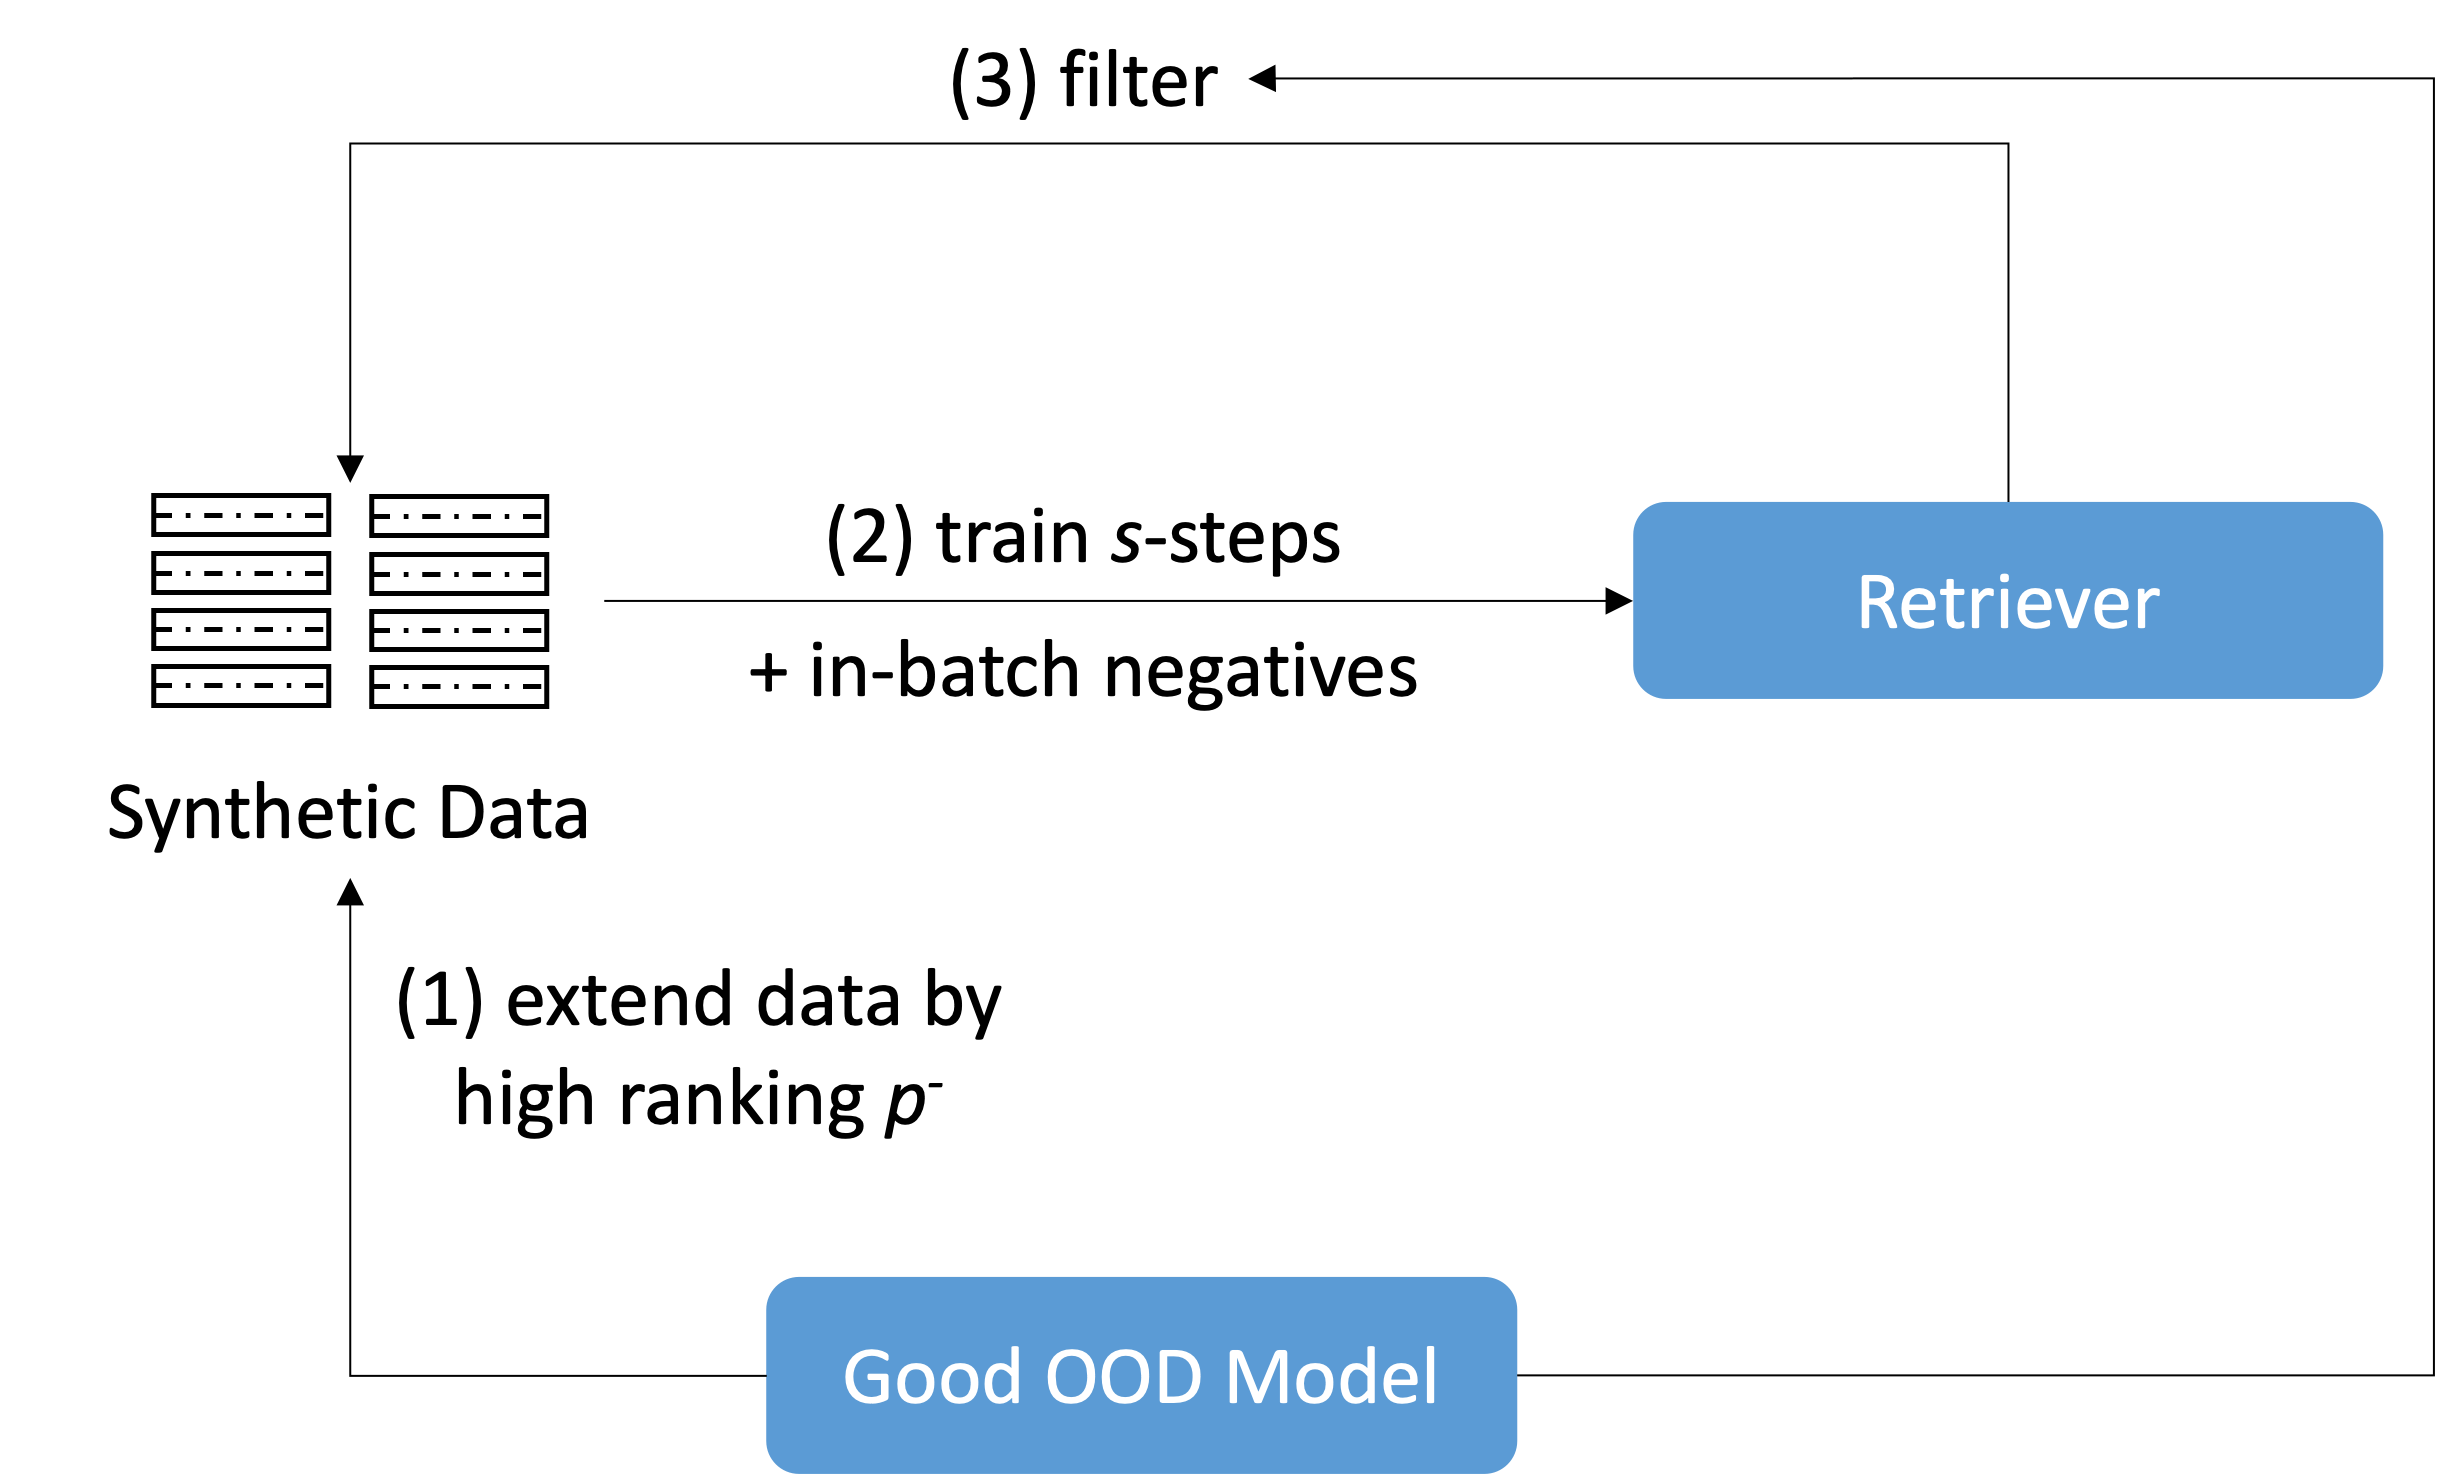
\includegraphics[width=0.8\textwidth]{Grafiken/Training.png}
%     \caption{Fine-Tuning Process for Retriever}
%     \label{fig:retriever-fine-tuning} 
% \end{figure}

% A crucial aspect of this fine-tuning approach is the utilization of an already well-performing out-of-domain retriever as a baseline. This baseline retriever can distill its knowledge into the retriever undergoing training. For example, \gls{dpr} used BM25, while ColBERTv2 employed MiniLM \cite{wang_multi-passage_2019}, a 22M-parameter Interaction-based retriever. A useful guideline for selecting the model is to consult the BEIR leaderboard.

% In the first step, the \gls{ood} model must retrieve the top $k$ passages, denoted as $p_i$, for each synthetic $(q_s,p^{+})$ pair. To generate numerous high-quality negative triples, denoted as $(q_s, p^{+}, p^{-})$, for every retrieved passage $p_i$ (where $p_i \neq p^{+}$), the triple $(q_s, p^{+}, p_i)$ is added to the training dataset.

% In the second step, the target retriever is trained for $s$ iterations. The loss function employed is the negative log likelihood, as defined in Section \ref{subsec:qa_retrieval}. During training, in-batch negatives are utilized. Let $Q$ and $P$ represent the $(B \times d)$ matrices of question and passage embeddings in a batch of size $B$. The matrix $S = Q P^{T}$ contains rows where each corresponds to a question paired with all other passages in the batch. The passages from all the other data points act as negatives for the question $q$.

% In the third step, the synthetic dataset is subjected to filtering. PROMPTAGATOR demonstrated promising results of filtering data by a network trained on the data. For this filtering process, retrieval is performed using both the newly trained model and the \gls{ood} model for a question $q_s$. If neither model retrieves the corresponding passage $p^{+}$ for the synthetic question within their top $k$, that question is removed from the dataset.

% Steps two and three are repeated once during fine-tuning.
% \subsection{Read}
% \label{subsec:read}

% \textbf{Out-of-Domain Readers:} There exists no benchmark for the application of zero-shot or \gls{ood} Readers. As Pereira et. al. \cite{pereira_visconde_2022} point out in their experimental results, the zero-shot performance of \gls{llm}s as Generative Readers is state-of-the-art and thus needs no fine-tuning and can even perform in a zero-shot setting. Luo et. al. \cite{luo_choose_2022} also pointed out, that the \gls{ood} performance of Extractive Readers is higher than the of Generative ones, when it comes to \gls{prlm}. Threfore a good \gls{ood} model choice is UnifiedQA-v2 \cite{khashabi_unifiedqa-v2_2022}, which is based on T5 \cite{raffel_exploring_2023} and was trained on 20 diverse datasets.

% \noindent\textbf{Fine-Tuning Readers:} Extractive Readers depend on datasets of the form $(q, c, a_span)$, whereas $q$ is a question, $c$ the context and $a_span$ an indication of which tokens of $c$ correspond to the desired answer. Similar for Generative Readers, which need $(q, c, a)$ datasets, whreas $a$ is just a text based answer to question $q$. The training process for the reader is easier and more straightforward as for the retriever. Given the already filtered synthetic trainings dataset, this can be used for training of the reader.

% \subsection{Orchestration}
% \label{subsec:qa_orchestration}

% Similar to \gls{r2d2}\cite{fajcik_r2-d2_2021} and LaPraDoR \cite{xu_laprador_2022} and others, an orchestration of retrievers and readers will be adopted in order to achieve highest \gls{ood} performance. This involves the following steps:

% \begin{enumerate}
%     \item \textit{Retrieval:} The $k$-top identified passages $P = \{p_1, p_2, \ldots, p_k\}$ are retrieved for a given question $q$ receive a similarity indication $\text{sim}(q,p_k)$ by the retriever. Next to this score, the BM25 score is calculated $BM25(q,p_k)$. The final score is calculated as the weighting of the similarity by BM25:     $score(q, d) = sim(q, d) \cdot BM25(q, d)$
%     \item \textit{Reader:} As for the Reader two readers will be executed at the same time: An extractive and one generative reader. Both 

% \end{enumerate}


% \section{Conversational Question Answering System}
% \label{sec:conv-qa-system}